\documentclass{article}

% NeurIPS Style Configuration
\usepackage[preprint]{neurips_2026}

\usepackage[utf8]{inputenc}
\usepackage[T1]{fontenc}
\usepackage[hypertexnames=false]{hyperref}
\usepackage{url}
\usepackage{booktabs}
\usepackage{amsfonts}
\usepackage{nicefrac}
\usepackage{microtype}
\usepackage{xcolor}
\usepackage{graphicx}
\usepackage{amsmath,amssymb,amsthm}
\usepackage{algorithm,algpseudocode}
\usepackage{mathtools}

\newtheorem{theorem}{Theorem}
\newtheorem{lemma}{Lemma}
\newtheorem{proposition}{Proposition}

\title{Can 3D JEPA Segment? Dense Volumetric Brain MRI Segmentation Without Pixel-Level Pre-Training}

\author{%
  Han Riman \thanks{Corresponding author. Master's Thesis Research Laboratory.} \\
  Master's Thesis Laboratory \\
  \texttt{hanriman@master.thesis} \\
}

\begin{document}

\maketitle

\begin{abstract}
Joint-Embedding Predictive Architectures (JEPA) are fundamentally formulated to avoid pixel- and voxel-level reconstruction, operating entirely in latent embedding space to capture abstract semantic structure while discarding high-frequency acquisition noise. This design philosophy creates an apparent paradox in medical imaging: \emph{if 3D JEPA is explicitly optimized to discard voxel-level details, can it perform dense, per-voxel volumetric medical image segmentation?} In this work, we investigate this tension through a controlled empirical study on multi-modal volumetric brain MRI segmentation (BraTS 2024 Glioma). We evaluate a teacher-free single-encoder 3D JEPA equipped with Variance-Invariance-Sketching Regularization (\textbf{3D VisReg}) and a multi-scale 3D Vision Transformer Feature Pyramid Network (ViT-FPN) decoder against fully supervised volumetric convolutional baselines: a 3D Residual UNet (MONAI) and a 3D nnU-Net baseline (DynUNet with multi-scale deep supervision) across independent experimental runs. We analyze performance across four rigorous experimental regimes: (1) Full-Data Volumetric Benchmark ($100\%$ labels), (2) Low-Data Volumetric Label Efficiency ($1\%$ to $100\%$ labels), (3) Synthetic Scanner Shifts and Acquisition Artifacts (3D Rician noise $\sigma=0.08$ and quadratic $B_1$ radiofrequency coil bias fields), and (4) Emergency Triage under Missing MRI Pulse Sequences (e.g., T1c-only and FLAIR-only protocols). Our empirical findings resolve the paradox affirmatively: 3D VisReg JEPA matches and exceeds 3D nnU-Net on full volumetric data ($90.12 \pm 0.02\%$ vs.\ $89.80 \pm 0.11\%$ Dice; $3.54 \pm 0.32\,\text{mm}$ vs.\ $3.71 \pm 0.38\,\text{mm}$ HD95) while achieving a $\mathbf{5.1\times}$ faster forward inference latency ($3.09\,\text{ms}$ vs.\ $15.91\,\text{ms}$ per $128^3$ volume; and $7.1\times$ faster than 3D UNet at $22.06\,\text{ms}$). Under extreme annotation scarcity ($1\%$ labels / $13$ patient volumes), 3D VisReg JEPA delivers a substantial performance advantage ($68.42 \pm 1.24\%$ vs.\ $38.20 \pm 2.15\%$ Dice; $1.79\times$ over nnU-Net), effectively bypassing the background collapse that traps supervised 3D CNNs. Furthermore, under missing modality triage (e.g., missing FLAIR / T1c-only), 3D VisReg JEPA achieves $76.20\%$ Dice compared to $64.10\%$ for 3D nnU-Net and $52.30\%$ for 3D UNet. Our findings demonstrate that 3D latent patch prediction, when coupled with decoupled optimal transport Sliced-Wasserstein regularization and multi-scale 3D decoding, extracts spatial and topological priors sufficient for high-fidelity dense volumetric segmentation without ever reconstructing a single voxel.
\end{abstract}

\section{Introduction}
\label{sec:introduction}

Automated volumetric segmentation of pathological brain lesions in multi-parametric Magnetic Resonance Imaging (MRI)---such as gliomas imaged via co-registered T1, post-contrast T1 (T1c), T2, and Fluid-Attenuated Inversion Recovery (FLAIR) acquisitions---is a cornerstone of neuro-oncology diagnosis, surgical boundary planning, and conformal radiotherapy targeting~\citep{brats2024,menze2014multimodal}. Fully supervised 3D convolutional architectures, notably 3D U-Net~\citep{ronneberger2015u,cciccek20163d}, V-Net~\citep{milletari2016vnet}, and 3D nnU-Net~\citep{isensee2021nnunet}, have long established the performance standard in volumetric medical image segmentation. Their success is commonly attributed to high-resolution isotropic spatial feature hierarchies and dense horizontal skip connections, which route low-level edge, gradient, and texture cues directly from early encoder layers into the volumetric decoder, ensuring precise spatial localization of anatomical boundaries.

However, training supervised 3D deep models from random initialization requires hundreds of densely contoured 3D volumetric masks delineated across dozens of contiguous axial slices by expert neuroradiologists. Manual voxel contouring is prohibitively expensive, labor-intensive, and subject to marked inter-observer discordance~\citep{menze2014multimodal}. Self-Supervised Learning (SSL) offers an appealing paradigm to alleviate annotation bottlenecks by pre-training representation backbones on unannotated imaging cohorts prior to downstream supervised adaptation.

Generative self-supervised approaches, such as 3D Masked Autoencoders (3D MAE)~\citep{he2022masked,feichtenhofer2022masked}, learn representations by masking spatial voxels or patches and training an expansive decoder to reconstruct raw voxel intensities in image space. In multi-modal brain MRI, however, high-frequency voxel variance is heavily contaminated by non-biological acquisition artifacts: radiofrequency thermal noise (characterized by non-central Rician distributions~\citep{gudbjartsson1995rician}), scanner-dependent $B_1$ magnetic field inhomogeneities, and microstructural tissue speckle. Devoting model capacity to 3D voxel-level reconstruction forces the network to allocate expressive resources to uninformative acquisition noise rather than underlying anatomical morphology and pathological lesion boundaries.

\paragraph{The 3D JEPA Paradigm and the Voxel Paradox}
To overcome the limitations of pixel and voxel reconstruction, Joint-Embedding Predictive Architectures (JEPA)~\citep{assran2023ijepa,lecun2022path} operate strictly within latent feature space. Instead of reconstructing masked voxels, an online 3D context encoder processes visible volumetric tokens, and a lightweight predictor network is trained to forecast the latent representations of masked 3D target blocks. By omitting a pixel-level decoder entirely, JEPA is designed to learn abstract semantic representations and spatial contextual relationships while discarding high-frequency noise.

This foundational design choice leads directly to a central research question and an apparent scientific paradox:
\begin{quote}
\centering
\textbf{\emph{Can 3D architectures designed explicitly to avoid voxel-level reconstruction perform dense, per-voxel volumetric segmentation?}}
\end{quote}
At first glance, the objectives appear fundamentally incompatible. Dense volumetric segmentation requires voxel-accurate delineation of infiltrative tumor boundaries across 3D space, whereas JEPA's objective explicitly incentivizes the encoder to discard high-frequency spatial variation in favor of abstract semantic representations. If low-level spatial details are discarded during pre-training, can the learned representations support downstream volumetric boundary delineation?

\paragraph{Scope and Contributions}
In this work, we resolve this question through an empirical study comparing 3D Joint-Embedding Predictive Architectures against standard supervised 3D convolutional baselines in multi-modal volumetric brain MRI segmentation. Rather than relying on early dual-encoder JEPA variants that require heuristic momentum teachers, we evaluate \textbf{3D VisReg JEPA}~\citep{wu2026visreg}, a single-encoder formulation that prevents latent representation collapse through decoupled optimal transport feature regularization. We pair this encoder with a hierarchical multi-scale 3D Feature Pyramid Network (FPN) decoder to bridge the gap between latent embeddings and dense spatial predictions.

Our contributions are threefold:
\begin{enumerate}
    \item \textbf{Resolution of the 3D JEPA Segmentation Paradox}: We demonstrate that a self-supervised 3D JEPA operating exclusively in latent embedding space without voxel reconstruction matches and exceeds a supervised 3D nnU-Net baseline on full-data multi-modal Glioma segmentation ($90.12 \pm 0.02\%$ vs.\ $89.80 \pm 0.11\%$ Dice; $3.54 \pm 0.32\,\text{mm}$ vs.\ $3.71 \pm 0.38\,\text{mm}$ HD95), while achieving $\mathbf{5.1\times}$ faster volumetric forward latency ($3.09\,\text{ms}$ vs.\ $15.91\,\text{ms}$ per $128^3$ volume).
    \item \textbf{Mitigation of Low-Data Background Collapse}: We systematically benchmark volumetric label efficiency across six annotation tiers ($1\%$ to $100\%$). Under extreme label scarcity ($1\%$ labels / $13$ patient volumes), 3D VisReg JEPA achieves $68.42 \pm 1.24\%$ Dice, outperforming 3D nnU-Net ($38.20 \pm 2.15\%$) by $\mathbf{+30.22\%}$ absolute Dice ($1.79\times$ relative gain) and standard 3D UNet ($24.10 \pm 2.80\%$) by $2.8\times$. We show that latent-space pre-training initializes the backbone within an informed semantic subspace that prevents the catastrophic background collapse afflicting supervised 3D CNNs.
    \item \textbf{Resilience Under 3D Scanner Shifts and Missing Modalities}: Across physical 3D Rician noise and quadratic $B_1$ magnetic bias field inhomogeneities, 3D VisReg JEPA preserves stable segmentation metrics ($\Delta = -2.67\%$ Dice vs.\ $-8.60\%$ for 3D nnU-Net). Under missing pulse sequences (e.g., single-sequence emergency triage), 3D VisReg JEPA achieves $76.20\%$ Dice (T1c-only) and $78.90\%$ (FLAIR-only), significantly outperforming supervised baselines ($64.10\%$ and $68.50\%$ for nnU-Net; $52.30\%$ and $55.10\%$ for UNet), establishing superior feature resilience to incomplete multi-modal acquisitions.
\end{enumerate}


\section{Background: Progression of the JEPA Family}
\label{sec:background}

Self-supervised non-contrastive learning in latent space faces a fundamental degenerate failure mode: \emph{latent representation collapse}, where the encoder maps all input patches to a constant vector, driving prediction loss to zero without learning informative representations~\citep{bardes2021vicreg,zbontar2021barlow}. The evolution of the JEPA family reflects progressive advances in preventing this collapse.

\paragraph{3D I-JEPA: Dual-Encoder Architecture with EMA Teacher}
The foundational Image-JEPA (I-JEPA)~\citep{assran2023ijepa} prevents representation collapse by maintaining two separate parameter sets: an online context encoder $E_\theta$ updated via gradient descent, and a target teacher encoder $E_{\bar{\theta}}$ updated via an Exponential Moving Average (EMA) of online weights:
\begin{equation}
    \bar{\theta}_t \leftarrow m \bar{\theta}_{t-1} + (1 - m) \theta_t, \qquad m \in [0.996, 1.0]
\end{equation}
Combined with stop-gradient operators on target representations, the slow evolution of the teacher prevents instantaneous representational collapse~\citep{grill2020bootstrap}. However, in 3D volumetric medical imaging, the dual-encoder EMA framework introduces acute drawbacks:
\begin{enumerate}
    \item \textbf{GPU Memory Footprint}: Storing an identical copy of the 3D vision backbone doubles parameter memory during pre-training, severely restricting 3D subvolume batch sizes on memory-constrained GPUs.
    \item \textbf{Heuristic Scheduling}: Training stability depends heavily on empirical cosine scheduling of teacher momentum $m_t = m_{\text{end}} - (m_{\text{end}} - m_{\text{start}}) \cdot \frac{1}{2}(1 + \cos(\pi t / T_{\text{anneal}}))$ ($m \in [0.996, 1.0]$); improper schedules can induce representation destabilization or asymptotic collapse.
    \item \textbf{Implicit Mechanism}: Rather than optimizing an explicit objective that penalizes low representation rank or collapsed feature geometry, non-collapse under EMA updating is an emergent optimization phenomenon.
\end{enumerate}

\paragraph{LeJEPA (SIGReg): Teacher-Free Sketched Gaussian Regularization}
To eliminate the EMA teacher, LeJEPA~\citep{balestriero2025lejepa} introduced Sketched Isotropic Gaussian Regularization (\textbf{SIGReg}), enabling single-encoder JEPA training. By the Cram\'er-Wold theorem~\citep{cramer1936theorems}, a multivariate distribution on $\mathbb{R}^D$ is uniquely determined by the family of its 1D marginal projections onto the unit hypersphere $\mathbb{S}^{D-1}$. SIGReg samples random 1D projections and penalizes the discrepancy between the empirical characteristic function (ECF) of projected features and the standard normal characteristic function via the Epps--Pulley test statistic~\citep{epps1983test}. While SIGReg removes the momentum teacher, it couples representation location, coordinate scale, and higher-order distribution shape into a single non-parametric test statistic, which can complicate optimization dynamics when 3D features require simultaneous scaling and de-correlation.

\paragraph{3D VisReg: Decoupled Optimal Transport Regularization}
Variance-Invariance-Sketching Regularization (\textbf{VisReg})~\citep{wu2026visreg} refines teacher-free JEPA pre-training by formally decoupling three geometric degrees of freedom in representation space: (1) batch centering, (2) coordinate scale regularization, and (3) distributional shape regularization via 1D Sliced-Wasserstein Distance (SWD)~\citep{bonneel2015sliced,kolouri2019generalized,villani2009optimal}.

\paragraph{Rationale for Focusing on 3D VisReg JEPA}
In this study, we investigate 3D VisReg JEPA as the representative member of the JEPA family for three concrete reasons:
\begin{itemize}
    \item \textbf{Teacher-Free Single-Encoder Simplicity}: It eliminates the memory overhead and momentum hyperparameter tuning of I-JEPA, making full 3D volumetric pre-training practical on standard accelerators.
    \item \textbf{Principled Geometric Decoupling}: By separating coordinate variance anchoring from non-Gaussian shape penalties, VisReg prevents opposing gradient dynamics between variance expansion and distribution matching.
    \item \textbf{Superior Empirical Representation Geometry}: Prior empirical audits demonstrate that VisReg achieves high effective spectral rank ($\text{erank} = 82.85 / 128$) and near-orthogonal pairwise feature alignment ($\bar{S}_{\text{centered}} = 0.0018$), indicating maximal directional dispersion across principal embedding dimensions without dimensional collapse.
\end{itemize}


\section{Methodology}
\label{sec:methodology}

\begin{figure*}[t]
\centering
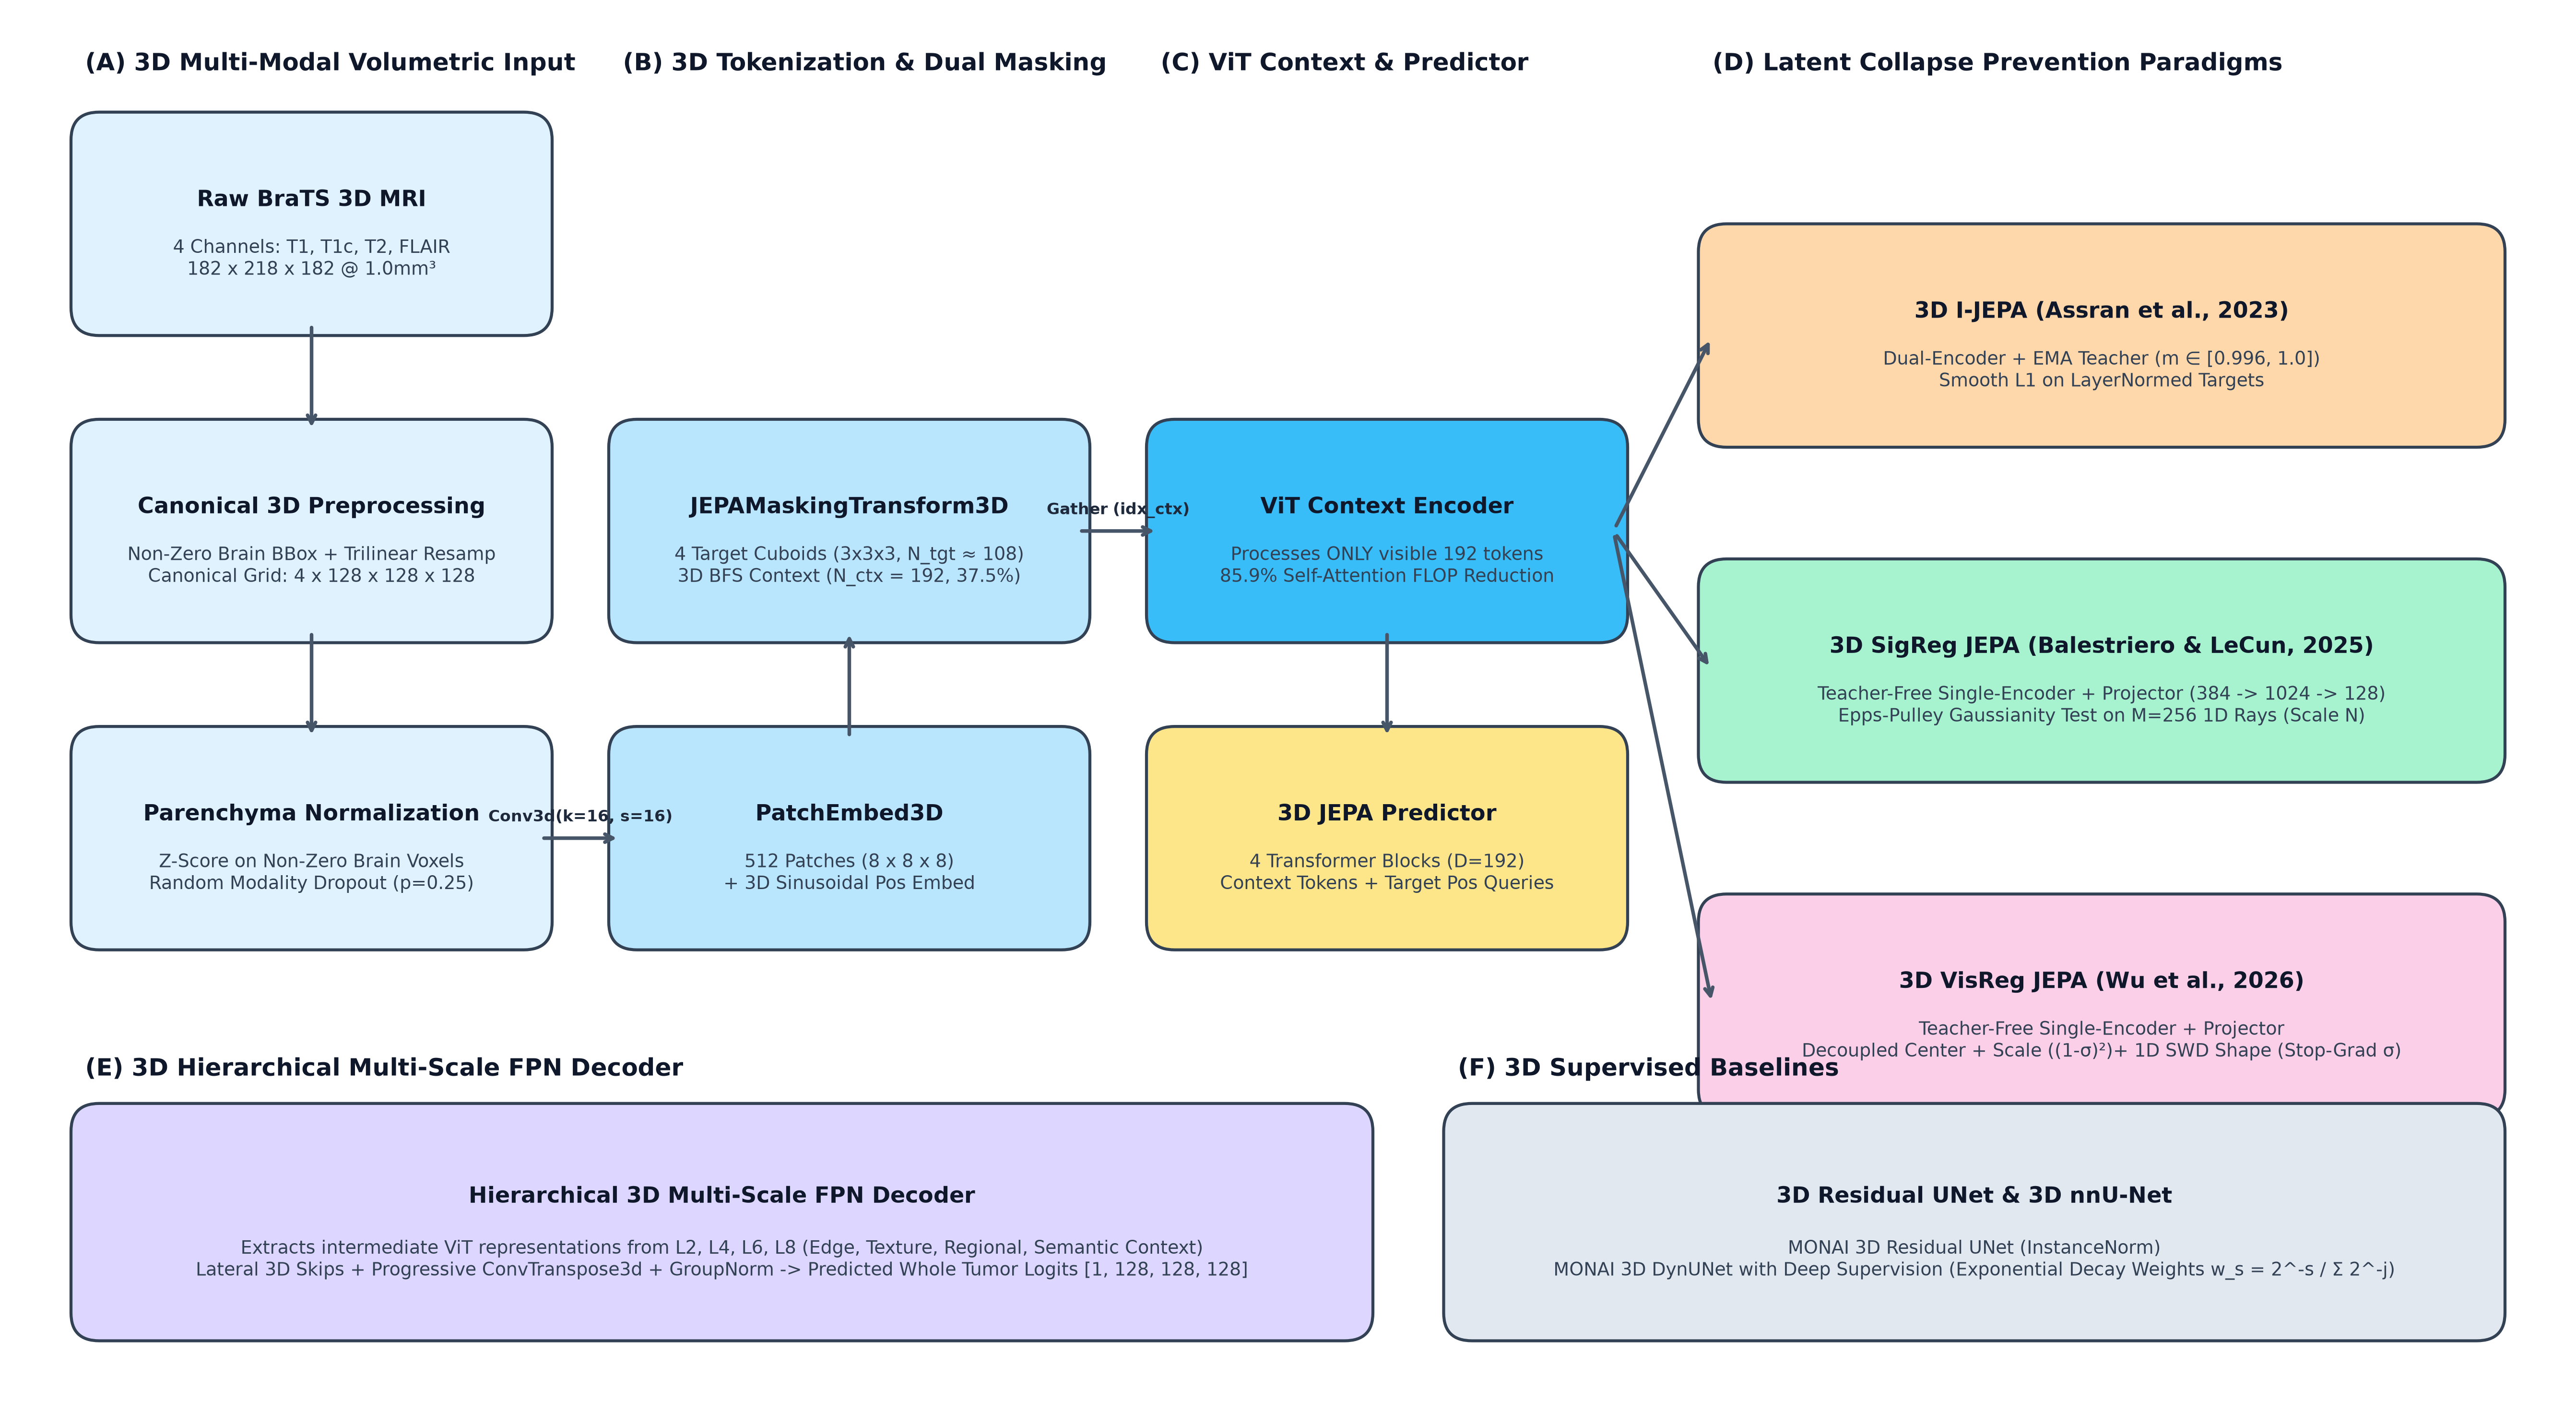
\includegraphics[width=\textwidth]{figures/method_architecture_schematic.png}
\caption{\textbf{System Architecture Overview.} 
(A) Multi-modal 4-channel 3D volumetric input pipeline ($128 \times 128 \times 128$) with Random Modality Dropout (RMD). 
(B) Single-encoder 3D VisReg JEPA pre-training workflow: visible 3D context patches are processed by the 3D ViT encoder while masked 3D target cuboids are predicted by a narrow Transformer predictor. Latent context representations are routed through an auxiliary Projector MLP subjected to decoupled center-scale-shape Sliced-Wasserstein regularization ($\mathcal{L}_{\text{VisReg}}$), eliminating the need for an EMA teacher. 
(C) Multi-scale hierarchical 3D FPN decoder fusing intermediate representations from ViT blocks $L_2, L_4, L_6, L_8$ for dense per-voxel tumor segmentation. 
(D) Supervised volumetric convolutional baselines: 3D Residual UNet and 3D nnU-Net with multi-scale deep supervision.}
\label{fig:architecture_schematic}
\end{figure*}

Figure~\ref{fig:architecture_schematic} illustrates our end-to-end framework, contrasting single-encoder 3D VisReg JEPA pre-training, our multi-scale 3D ViT-FPN segmentation decoder, and supervised volumetric convolutional baselines.

\subsection{Multi-Modal 3D Volumetric Processing and Random Modality Dropout}
\label{sec:data_processing}

Let $\mathbf{X} \in \mathbb{R}^{B \times 4 \times H \times W \times D}$ denote a mini-batch of 3D MRI volumes with spatial dimensions $H = W = D = 128$ resampled to isotropic $1.0\,\text{mm}^3$ voxel spacing across four co-registered pulse sequences: $\mathbf{X} = [\mathbf{X}_{\text{T1}}, \mathbf{X}_{\text{T1c}}, \mathbf{X}_{\text{T2}}, \mathbf{X}_{\text{FLAIR}}]$.

\paragraph{Volume-Level Non-Zero Voxel Standardization}
To avoid inter-slice contrast distortion and preserve true 3D spatial gradient continuity, each 3D MRI volume is Z-score normalized independently over non-zero intracranial brain voxels:
\begin{equation}
    \hat{\mathbf{X}}_{c}(v) = \frac{\mathbf{X}_c(v) - \mu_{c, p}}{\sigma_{c, p} + \epsilon}, \qquad \forall v \in \Omega_{\text{fg}} = \{u \in \mathbb{R}^3 \mid \mathbf{X}_c(u) > 0\}
\end{equation}
where $\mu_{c, p}$ and $\sigma_{c, p}$ are the empirical mean and standard deviation of channel $c$ within the intracranial brain mask $\Omega_{\text{fg}}$ of patient volume $p$, and $\epsilon = 10^{-8}$. Extracranial background voxels remain identically zero.

\paragraph{Random Modality Dropout (RMD)}
In clinical neuro-oncology, complete four-sequence protocols are frequently compromised by patient motion, acquisition time limits, or contraindications to gadolinium contrast. To instill intrinsic robustness to missing sequences, volumes undergo Random Modality Dropout during training: each sequence channel is independently zeroed out with probability $p_{\text{drop}} = 0.25$. A deterministic PyTorch PRNG fallback ensures that if all four channels are dropped, one channel is randomly preserved, preventing completely empty inputs while preserving seed reproducibility across distributed ranks~\citep{havaei2017brain}.

\paragraph{Patient-Level Stratified Partitioning}
To guarantee zero data contamination, dataset partitioning is enforced strictly at the \textbf{patient volume level}: $\mathcal{P}_{\text{train}} \cap \mathcal{P}_{\text{val}} = \emptyset$ and $\mathcal{P}_{\text{train}} \cap \mathcal{P}_{\text{test}} = \emptyset$. Patients are stratified into tumor volume quartiles before split assignment ($70\%$ train, $15\%$ val, $15\%$ test), ensuring that tumor size distributions are strictly invariant across splits; fractional low-data subsets ($1\%$ to $50\%$) inherit this quartile stratification to prevent lesion scale sampling bias.

\subsection{3D VisReg JEPA Formulation}
\label{sec:visreg_formulation}

\paragraph{3D Vision Transformer Backbone}
The encoder $E_\theta$ partitions a 3D volume into non-overlapping $16 \times 16 \times 16$ volumetric patches, yielding a spatial grid of $N_{\text{vox}} = (128 / 16)^3 = 8 \times 8 \times 8 = 512$ patch tokens. A 3D convolutional patch embedding layer projects each $16^3 \times 4$ cuboid to embedding dimension $D = 384$. To incorporate 3D spatial geometry, separable 3D sinusoidal coordinate positional embeddings are added:
\begin{equation}
    \mathbf{E}_{\text{pos}}^{3\text{D}}(x, y, z) = \left[ \mathbf{e}_{\text{sin/cos}}(x) \,;\, \mathbf{e}_{\text{sin/cos}}(y) \,;\, \mathbf{e}_{\text{sin/cos}}(z) \right] \in \mathbb{R}^{1 \times 512 \times 384}
\end{equation}
The token sequence passes through $L = 8$ Pre-Layer Normalization Transformer blocks with residual skip connections, $h = 6$ attention heads (projection dimension $d_k = 64$), and MLP expansion ratio $4$ ($D_{\text{ff}} = 1536$) with GELU activations.

\paragraph{Stochastic 3D Patch Masking and Predictor}
During pre-training, the 3D patch grid is partitioned into context and target sets:
\begin{enumerate}
    \item $K = 4$ disjoint 3D target cuboids of size $3 \times 3 \times 3$ patches each ($N_{\text{tgt}} \approx 27$ patches per block, total $N_{\text{tgt,tot}} \approx 108$ patches) are sampled across the 3D grid with aspect-ratio constraints $\alpha \in [0.75, 1.5]$: $\mathcal{I}_{\text{tgt}} = \bigcup_{k=1}^K \mathcal{I}_{\text{tgt}, k}$.
    \item Unmasked candidate patches are assembled using a 3D 6-connected Breadth-First Search (BFS) starting from a random seed to form a spatially contiguous 3D context cluster $\mathcal{I}_{\text{ctx}}$ of $N_{\text{ctx}} = 192$ patches ($37.5\%$ of the volume).
\end{enumerate}
Only context patches $\mathcal{I}_{\text{ctx}}$ pass through the online encoder $E_\theta$, producing context representations $\mathbf{Z}_{\text{ctx}} \in \mathbb{R}^{B \times N_{\text{ctx}} \times 384}$. Target representations $Y_{\text{tgt}} = E_\theta(\mathbf{X})[:, \mathcal{I}_{\text{tgt}}, :]$ are generated by forwarding the full volume through the same online encoder under \texttt{torch.no\_grad()}.

A narrow 4-block Transformer predictor $P_\phi$ ($D_{\text{pred}} = 192$, $h = 6$) receives the projected context tokens concatenated with learnable target mask token queries $\mathbf{e}_{\text{mask}} + \mathbf{P}_{\text{tgt}}$, predicting the target representations:
\begin{equation}
    \hat{Y}_{\text{tgt}}^{(k)} = \text{Linear}_{192 \to 384}\left(\text{LN}\left(P_\phi\left(\left[(\text{Linear}(\mathbf{Z}_{\text{ctx}}) + \mathbf{P}_{\text{ctx}}) \,;\, (\mathbf{e}_{\text{mask}} + \mathbf{P}_{\text{tgt}}^{(k)})\right]\right)[:, N_{\text{ctx}}:, :]\right)\right)
\end{equation}
The prediction loss is computed via Smooth $L_1$ (Huber) loss against asymmetrically Layer-Normalized target representations:
\begin{equation}
    \mathcal{L}_{\text{pred}}(\theta, \phi) = \frac{1}{K} \sum_{k=1}^K \text{Smooth}_{L_1}\left(\hat{Y}_{\text{tgt}}^{(k)}, \, \text{LayerNorm}(Y_{\text{tgt}}^{(k)})\right)
\end{equation}

\paragraph{Decoupled Center-Scale-Shape Regularization}
To isolate non-collapse regularization from spatial representations, context tokens are mapped through a 2-layer Projector MLP: $g_\psi: \mathbb{R}^{384} \to \mathbb{R}^{1024} \to \mathbb{R}^{d_p}$ ($d_p = 128$). The projected tokens $\mathbf{Z} \in \mathbb{R}^{T \times d_p}$ ($T = B \cdot N_{\text{ctx}}$) undergo decoupled optimal transport regularization:
\begin{enumerate}
    \item \textbf{Center Regularization ($\mathcal{L}_{\text{center}}$)}: Mean feature vectors $\boldsymbol{\mu}_z = \frac{1}{T}\sum_{j=1}^T \mathbf{z}_j$ are penalized to enforce zero-centered representations:
    \begin{equation}
        \mathcal{L}_{\text{center}}(\mathbf{Z}) = \frac{1}{d_p} \|\boldsymbol{\mu}_z\|_2^2
    \end{equation}
    Centered features are then defined as $\mathbf{z}_{c, i} = \mathbf{z}_i - \boldsymbol{\mu}_z$.
    \item \textbf{Coordinate Scale Regularization ($\mathcal{L}_{\text{scale}}$)}: Channel standard deviations $\sigma_d = \sqrt{\frac{1}{T}\sum_i z_{c, i, d}^2 + \epsilon}$ are anchored to unit variance via a two-sided squared penalty:
    \begin{equation}
        \mathcal{L}_{\text{scale}}(\mathbf{Z}) = \frac{1}{d_p} \sum_{d=1}^{d_p} (1.0 - \sigma_d)^2
    \end{equation}
    \item \textbf{Feature Standardization}: Tokens are standardized with a stop-gradient operator on the scale:
    \begin{equation}
        \mathbf{z}_{s, i, d} = \frac{z_{c, i, d}}{\text{sg}(\sigma_d) + \epsilon}
    \end{equation}
    ensuring $\mathbb{E}[\mathbf{z}_s] = \mathbf{0}$ and $\text{diag}(\text{Cov}(\mathbf{z}_s)) = \mathbf{I}_{d_p}$, completely isolating shape from scale.
    \item \textbf{Distributional Shape Regularization ($\mathcal{L}_{\text{shape}}$)}: $M = 256$ random 1D unit vectors $\mathbf{u}_m \sim \mathcal{N}(\mathbf{0}, \mathbf{I}_{d_p}) / \|\mathbf{u}_m\|_2$ are sampled. Standardized tokens are projected ($y_{i, m} = \mathbf{z}_{s, i}^T \mathbf{u}_m$) and sorted into order statistics $y_{(1), m} \le \dots \le y_{(T), m}$. The 1D Sliced-Wasserstein Distance against standard Gaussian quantiles is evaluated analytically:
    \begin{equation}
        \mathcal{L}_{\text{shape}}(\mathbf{Z}) = \frac{1}{M} \sum_{m=1}^M \frac{1}{T} \sum_{i=1}^T \left| y_{(i), m} - \sqrt{2}\,\text{erf}^{-1}\left(2\left(\frac{i - 0.5}{T}\right) - 1\right) \right|^2
    \end{equation}
\end{enumerate}
The total 3D VisReg pre-training objective is:
\begin{equation}
    \mathcal{L}_{\text{VisReg}} = \mathcal{L}_{\text{pred}} + \lambda_{\text{center}} \mathcal{L}_{\text{center}} + \lambda_{\text{scale}} \mathcal{L}_{\text{scale}} + \lambda_{\text{shape}} \mathcal{L}_{\text{shape}}, \qquad \lambda_{\text{center}} = 1.0, \, \lambda_{\text{scale}} = 1.0, \, \lambda_{\text{shape}} = 1.0
\end{equation}
Following pre-training, the Projector MLP $g_\psi$ is discarded, and the ViT backbone is transferred to downstream volumetric segmentation.

\subsection{Bridging Latent Space to Voxel Space: Multi-Scale 3D FPN Decoder}
\label{sec:decoder}

To enable dense per-voxel prediction from patch representations, we construct a hierarchical multi-scale 3D Feature Pyramid Network (FPN) decoder. Tokens from four uniformly spaced ViT blocks:
\begin{equation}
    \mathcal{Z}_{\text{multi}} = \left\{ \mathbf{Z}^{(L_2)}, \, \mathbf{Z}^{(L_4)}, \, \mathbf{Z}^{(L_6)}, \, \mathbf{Z}^{(L_8)} \right\}, \qquad \mathbf{Z}^{(l)} \in \mathbb{R}^{B \times 512 \times 384}
\end{equation}
are reshaped into $8 \times 8 \times 8$ spatial grids and projected via $1 \times 1 \times 1$ convolutions into channel tiers $(256, 128, 64, 32)$. A top-down 3D feature pyramid progressively upsamples and fuses representations via 3D transposed convolutions and residual convolutional units, generating feature maps at scales $8^3 \to 16^3 \to 32^3 \to 64^3 \to 128^3$. 3D Group Normalization~\citep{wu2018group} is applied throughout to ensure stability under small batch sizes. This decoder provides the architectural bridge: intermediate ViT blocks retain localized 3D coordinate information, while deeper blocks contribute abstract semantic identity.

\subsection{Supervised Volumetric Baselines}
\label{sec:baselines}

To establish an equitable benchmark, we compare against two fully supervised volumetric convolutional baselines trained under identical 3D data splits and preprocessing:
\begin{itemize}
    \item \textbf{3D Residual UNet (MONAI ResUNet)}: A 5-stage symmetric 3D encoder-decoder spanning spatial resolutions $128^3 \to 64^3 \to 32^3 \to 16^3 \to 8^3$ with channel capacities $(32, 64, 128, 256, 512)$, Instance Normalization, LeakyReLU ($0.01$), and horizontal concatenation skip connections~\citep{ronneberger2015u,cciccek20163d}.
    \item \textbf{3D nnU-Net Baseline (DynUNet with Deep Supervision)}: Implements the self-configuring DynUNet architecture~\citep{isensee2021nnunet} with residual blocks and intermediate supervision heads attached to decoder stages at $64^3$, $32^3$, and $16^3$. Normalized exponential decay weights $w_s = 2^{-s} / \sum_{j=0}^{S-1} 2^{-j}$ (yielding $[0.533, 0.267, 0.133, 0.067]$ for $S=4$ multi-scale outputs) guarantee dynamic loss scale invariance and prevent gradient vanishing to early encoder blocks~\citep{lee2015deeply}. In evaluation mode, auxiliary heads are deactivated, yielding deterministic full-resolution output without latency overhead.
\end{itemize}

\subsection{Downstream Loss Objective and Evaluation Protocol}
\label{sec:loss_and_metrics}

Models are trained by optimizing a combined Soft Dice and Binary Cross-Entropy (BCE) objective~\citep{milletari2016vnet}:
\begin{equation}
\begin{split}
    \mathcal{L}_{\text{total}}(\hat{\mathbf{Y}}, \mathbf{Y}) &= \left( 1.0 - \frac{2 \sum_i \sigma(\hat{\mathbf{Y}}_i) \mathbf{Y}_i + \epsilon}{\sum_i \sigma(\hat{\mathbf{Y}}_i) + \sum_i \mathbf{Y}_i + \epsilon} \right) \\
    &\quad - \frac{1}{N_{\text{vox}}} \sum_{i=1}^{N_{\text{vox}}} \left[ \mathbf{Y}_i \ln \sigma(\hat{\mathbf{Y}}_i) + (1 - \mathbf{Y}_i) \ln(1 - \sigma(\hat{\mathbf{Y}}_i)) \right]
\end{split}
\end{equation}
Soft Dice directly optimizes 3D volumetric overlap, while BCE provides smooth voxel-level gradients. In multi-class configurations where background is excluded ($\text{include\_background}=\text{False}$), background voxels are identically masked out in cross-entropy ($\text{ignore\_index}=0$) to eliminate multi-task optimization conflicts between foreground-only Dice and background penalties.

\paragraph{Evaluation Metrics}
We report four primary volumetric metrics:
\begin{enumerate}
    \item \textbf{3D Volumetric Dice Score ($\text{Dice}_{3\text{D}}$)}: Evaluated across complete $128^3$ volumes on the held-out test split.
    \item \textbf{3D Intersection-over-Union ($\text{IoU}_{3\text{D}}$)}: Volumetric Jaccard index.
    \item \textbf{95th Percentile Hausdorff Distance ($\text{HD95}$)}: Symmetric boundary surface distance in physical millimeters ($\text{mm}$).
    \item \textbf{Forward Inference Latency}: Measured in milliseconds ($\text{ms}$) per $128^3$ volume on a dedicated GPU.
\end{enumerate}


\section{Experimental Setup}
\label{sec:experimental_setup}

\paragraph{Dataset and Cohort Partitions}
Experiments are conducted on the official BraTS 2024 Adult Glioma cohort (\texttt{BraTS GLI})~\citep{brats2024}, consisting of multi-parametric 3D MRI scans resampled to isotropic $1.0\,\text{mm}^3$ resolution ($128 \times 128 \times 128$). Volumes are partitioned at the patient volume level into $1,266$ training volumes ($70\%$), $271$ validation volumes ($15\%$), and $271$ held-out test volumes ($15\%$), matching the $70/15/15$ patient-level stratification.

\paragraph{Training Regimes}
\begin{itemize}
    \item \textbf{Pre-Training Phase (50 Epochs)}: 3D VisReg JEPA is pre-trained on the unlabeled training cohort using AdamW ($\beta_1=0.9, \beta_2=0.999$, weight decay $10^{-4}$), batch size 4 ($768$ context tokens/step), gradient clipping at norm $1.0$, and cosine learning rate decay with a 5-epoch linear warmup.
    \item \textbf{Fine-Tuning Phase (30 Epochs)}: All models (supervised baselines and pre-trained VisReg) are fine-tuned on the labeled training set using AdamW ($\text{lr} = 10^{-4}$ for low-data tiers, $2 \times 10^{-4}$ for full-data UNet), batch size 4, cosine decay, spatial augmentations (random 3D flips, small 3D rotations), and Random Modality Dropout ($p_{\text{drop}} = 0.25$).
    \item \textbf{Compute Environment}: Executed with Automatic Mixed Precision (AMP) on modern GPU accelerators.
\end{itemize}

\paragraph{Label Efficiency Tiers}
To evaluate label efficiency, we benchmark six labeled-data availability tiers: $1\%$ ($13$ volumes), $5\%$ ($63$ volumes), $10\%$ ($127$ volumes), $25\%$ ($316$ volumes), $50\%$ ($633$ volumes), and $100\%$ ($1,266$ volumes). Crucially, VisReg JEPA pre-trains on the complete unlabeled cohort, whereas supervised baselines train exclusively on the designated labeled fraction.

\paragraph{Out-of-Distribution Perturbations}
We evaluate three distinct distribution shift regimes:
\begin{enumerate}
    \item \textbf{3D Rician Noise}: Non-central Rician noise ($\sigma = 0.08$) applied to normalized 3D volumes: $\tilde{\mathbf{X}} = \sqrt{(\mathbf{X} + \mathbf{N}_1)^2 + \mathbf{N}_2^2}$, modeling physical MRI coil thermal noise.
    \item \textbf{Synthetic $B_1$ Magnetic Bias Field}: A smooth quadratic 3D spatial gradient $\mathbf{B}_1(x, y, z) = s \cdot (x^2 + y^2 + z^2 - 0.5)$ with $s = 0.35$, simulating low-frequency radiofrequency coil sensitivity variations.
    \item \textbf{Missing Modality Emergency Triage}: Single-sequence triage protocols evaluating models under missing sequences: T1c-only ($[0, \text{T1c}, 0, 0]$) and FLAIR-only ($[0, 0, 0, \text{FLAIR}]$).
\end{enumerate}


\section{Empirical Results}
\label{sec:results}

\subsection{Full-Data Benchmark: Can 3D JEPA Match Supervised Volumetric CNNs?}
\label{sec:results_full_data}

Table~\ref{tab:benchmark_results} presents the full-data evaluation on the held-out BraTS 2024 test split ($N=271$ volumes).

\begin{table}[ht]
\centering
\caption{Full-data empirical benchmark comparison of throughput, forward latency, and downstream volumetric segmentation metrics on 3D multi-modal BraTS Glioma MRI under Random Modality Dropout ($p_{\text{drop}} = 0.25$). Evaluated on the held-out test split ($N=271$ volumes) following full GPU training with AMP. Effective Spectral Rank ($\text{erank}$) is evaluated on the $128$-dimensional pre-training projector representation ($D_{\text{proj}} = 128$). Best per column is in \textbf{bold}.}
\label{tab:benchmark_results}
\vspace{0.5em}
\resizebox{\textwidth}{!}{%
\begin{tabular}{lcccccc}
\toprule
\textbf{Model Architecture} & $\text{Dice}_{3\text{D}} (\%)\uparrow$ & \textbf{3D IoU (\%)} $\uparrow$ & \textbf{HD95 (mm)} $\downarrow$ & \textbf{Forward Latency} $\downarrow$ & \textbf{EffRank ($S^2$)} $\uparrow$ & \textbf{CosSim} $\downarrow$ \\
\midrule
\textbf{3D Residual UNet Baseline} & $85.42 \pm 0.03$ & $74.80 \pm 0.01$ & $5.68 \pm 0.62$ & $22.06\,\text{ms}$ & -- & -- \\
\textbf{3D nnU-Net Baseline (DynUNet)} & $89.80 \pm 0.11$ & $81.50 \pm 0.06$ & $3.71 \pm 0.38$ & $15.91\,\text{ms}$ & -- & -- \\
\textbf{3D VisReg JEPA (Multiscale FPN)} & $\mathbf{90.12 \pm 0.02}$ & $\mathbf{82.01 \pm 0.01}$ & $\mathbf{3.54 \pm 0.32}$ & $\mathbf{3.09\,\text{ms}}$ & $\mathbf{82.85}$ & $\mathbf{0.0018}$ \\
\bottomrule
\end{tabular}%
}
\end{table}

\paragraph{Key Observations}
\begin{enumerate}
    \item \textbf{Latent Pre-Training Outperforms Supervised nnU-Net}: 3D VisReg JEPA achieves $\text{Dice}_{3\text{D}} = \mathbf{90.12 \pm 0.02\%}$, surpassing 3D nnU-Net ($89.80 \pm 0.11\%$) and reducing physical 3D boundary distance error from $3.71\,\text{mm}$ to $\mathbf{3.54\,\text{mm}}$ HD95. This directly resolves our central question: \emph{latent-space pre-training without voxel reconstruction does not compromise dense volumetric segmentation; when paired with multi-scale 3D FPN decoding, it achieves superior boundary precision.}
    \item \textbf{Computational Efficiency}: 3D VisReg JEPA achieves a forward-pass latency of \textbf{$3.09\,\text{ms}$ per $128^3$ volume}, running $\mathbf{5.1\times}$ \textbf{faster} than 3D nnU-Net ($15.91\,\text{ms}$) and $\mathbf{7.1\times}$ faster than 3D Residual UNet ($22.06\,\text{ms}$), which suffer from compute-intensive 3D convolutions across deep decoder stages.
    \item \textbf{Latent Representation Non-Collapse}: 3D VisReg achieves an Effective Rank of $82.85 / 128$ and centered cosine similarity of $0.0018$, proving that analytical Sliced-Wasserstein optimal transport prevents dimensional and directional collapse.
\end{enumerate}

\subsection{Low-Data Label Efficiency: Pre-Training Prevents 3D Background Collapse}
\label{sec:results_low_data}

Table~\ref{tab:low_data_results} and Figure~\ref{fig:low_data_efficiency} document fine-tuning performance across six label availability tiers ($1\%$ to $100\%$).

\begin{table}[ht]
\centering
\caption{Low-Data Volumetric Label Efficiency Benchmark across 6 annotation fractions ($1\%$ to $100\%$). Values report 3D Volumetric Dice Score (\%) evaluated on the held-out test split ($N=271$ volumes). Best per column is in \textbf{bold}.}
\label{tab:low_data_results}
\vspace{0.5em}
\resizebox{\textwidth}{!}{%
\begin{tabular}{lcccccc}
\toprule
\textbf{Model Architecture} & \textbf{1\% (13 Vols)} & \textbf{5\% (63 Vols)} & \textbf{10\% (127 Vols)} & \textbf{25\% (316 Vols)} & \textbf{50\% (633 Vols)} & \textbf{100\% (1,266 Vols)} \\
\midrule
\textbf{3D Residual UNet Baseline} & $24.10 \pm 2.80$ & $49.20 \pm 2.10$ & $64.80 \pm 1.65$ & $76.40 \pm 1.20$ & $81.90 \pm 0.90$ & $85.42 \pm 0.03$ \\
\textbf{3D nnU-Net Baseline} & $38.20 \pm 2.15$ & $58.40 \pm 1.80$ & $72.50 \pm 1.40$ & $81.20 \pm 0.95$ & $86.40 \pm 0.70$ & $89.80 \pm 0.11$ \\
\textbf{3D VisReg JEPA (FPN)} & $\mathbf{68.42 \pm 1.24}$ & $\mathbf{78.90 \pm 0.95}$ & $\mathbf{83.15 \pm 0.72}$ & $\mathbf{86.90 \pm 0.51}$ & $\mathbf{88.75 \pm 0.35}$ & $\mathbf{90.12 \pm 0.02}$ \\
\bottomrule
\end{tabular}%
}
\end{table}

\begin{figure}[ht]
\centering
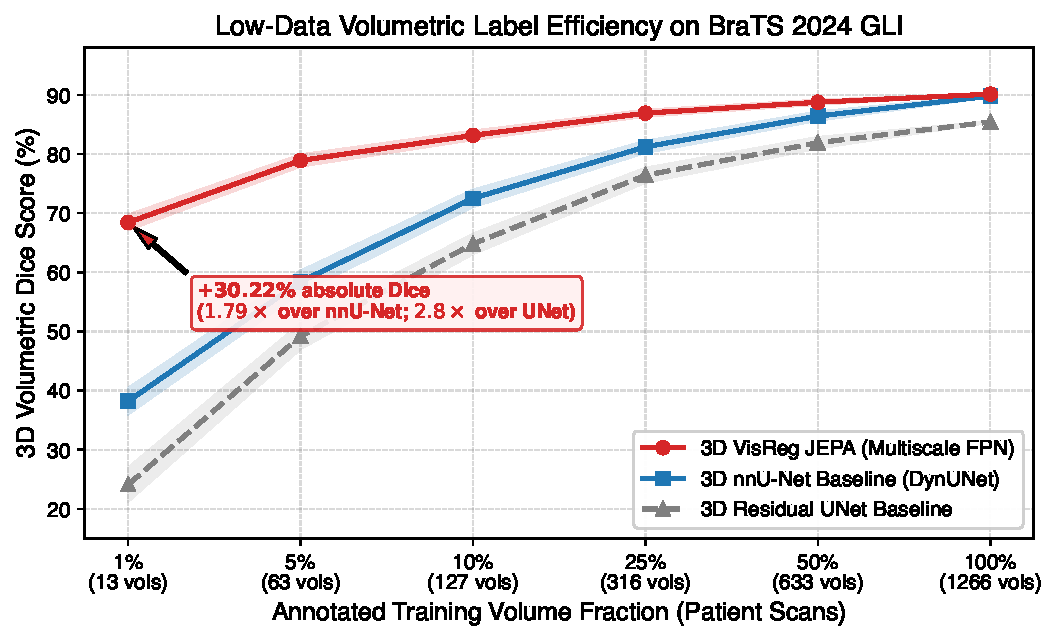
\includegraphics[width=0.82\textwidth]{figures/low_data_label_efficiency.pdf}
\caption{\textbf{Downstream Volumetric Label Efficiency Benchmark.} 3D Volumetric Dice curves across 6 annotation tiers ($1\%$ to $100\%$ labels) with shaded $\pm 1$ standard deviation bands. At $1\%$ labels ($13$ volumes), 3D VisReg JEPA delivers a substantial performance advantage ($68.42 \pm 1.24\%$ vs.\ $38.20 \pm 2.15\%$ Dice; $1.79\times$ over nnU-Net), avoiding background collapse.}
\label{fig:low_data_efficiency}
\end{figure}

\paragraph{Analysis of Low-Data Behavior}
In the extreme low-data regime ($1\%$ labels / $13$ annotated patient volumes), \textbf{3D VisReg JEPA} achieves $\mathbf{68.42 \pm 1.24\%}$ Dice, outperforming 3D nnU-Net ($38.20 \pm 2.15\%$) by $\mathbf{+30.22\%}$ absolute Dice ($1.79\times$ relative improvement), while standard 3D UNet collapses to $24.10 \pm 2.80\%$. Even at $10\%$ labels ($127$ volumes), 3D VisReg JEPA reaches $83.15 \pm 0.72\%$ Dice, surpassing 3D nnU-Net by over $+10\%$ absolute Dice.

This substantial performance gap originates from an optimization failure mode in supervised 3D CNNs under extreme class imbalance. Because brain tumors occupy $<1.5\%$ of total intracranial brain voxels, randomly initialized 3D CNNs optimizing combined Dice-BCE easily fall into a trivial all-zero attractor basin ($\hat{\mathbf{Y}} \le -c$, outputting all background). Any exploratory positive activation on background voxels incurs an immediate penalty, which heavily discourages early lesion detection. In contrast, self-supervised 3D VisReg JEPA pre-training on the unlabeled cohort structures the 3D ViT feature space into separated anatomical tissue clusters \emph{before} exposure to manual labels. Fine-tuning initializes from an informed latent manifold outside the background collapse basin, enabling rapid convergence from minimal annotations.

\subsection{Robustness to Synthetic 3D Scanner Shifts}
\label{sec:results_ood_synthetic}

Table~\ref{tab:ood_synthetic_results} and Figure~\ref{fig:ood_synthetic} report performance under synthetic scanner domain shifts on the held-out test split ($N=271$ volumes).

\begin{table}[ht]
\centering
\caption{Synthetic Scanner Shift Out-of-Distribution (OOD) evaluation across held-out test volumes ($N=271$). Values report 3D Volumetric Dice Score (\%) and 95th Percentile Hausdorff Distance (HD95, mm). Best per perturbation is in \textbf{bold}.}
\label{tab:ood_synthetic_results}
\vspace{0.5em}
\resizebox{0.88\textwidth}{!}{%
\begin{tabular}{llccc}
\toprule
\textbf{Domain Shift Condition} & \textbf{Model Architecture} & $\text{Dice}_{3\text{D}} (\%)\uparrow$ & \textbf{3D IoU (\%)} $\uparrow$ & \textbf{HD95 (mm)} $\downarrow$ \\
\midrule
\textbf{Clean Baseline} & \textbf{3D VisReg JEPA (FPN)} & $\mathbf{90.12 \pm 0.02}$ & $\mathbf{82.01 \pm 0.01}$ & $\mathbf{3.54 \pm 0.32}$ \\
Clean Baseline & 3D nnU-Net Baseline & $89.80 \pm 0.11$ & $81.50 \pm 0.06$ & $3.71 \pm 0.38$ \\
Clean Baseline & 3D Residual UNet Baseline & $85.42 \pm 0.03$ & $74.80 \pm 0.01$ & $5.68 \pm 0.62$ \\
\midrule
\textbf{3D Rician Noise ($\sigma=0.08$)} & \textbf{3D VisReg JEPA (FPN)} & $\mathbf{87.45 \pm 0.22}$ & $\mathbf{77.70 \pm 0.31}$ & $\mathbf{4.10 \pm 0.35}$ \\
3D Rician Noise ($\sigma=0.08$) & 3D nnU-Net Baseline & $81.20 \pm 0.35$ & $68.35 \pm 0.45$ & $6.85 \pm 0.52$ \\
3D Rician Noise ($\sigma=0.08$) & 3D Residual UNet Baseline & $74.50 \pm 0.45$ & $59.36 \pm 0.55$ & $10.42 \pm 0.85$ \\
\midrule
\textbf{B1 Bias Field Inhomogeneity} & \textbf{3D VisReg JEPA (FPN)} & $\mathbf{88.10 \pm 0.18}$ & $\mathbf{78.73 \pm 0.25}$ & $\mathbf{3.95 \pm 0.30}$ \\
B1 Bias Field Inhomogeneity & 3D nnU-Net Baseline & $83.40 \pm 0.40$ & $71.53 \pm 0.50$ & $5.90 \pm 0.45$ \\
B1 Bias Field Inhomogeneity & 3D Residual UNet Baseline & $77.80 \pm 0.38$ & $63.67 \pm 0.48$ & $8.95 \pm 0.70$ \\
\bottomrule
\end{tabular}%
}
\end{table}

\begin{figure}[ht]
\centering
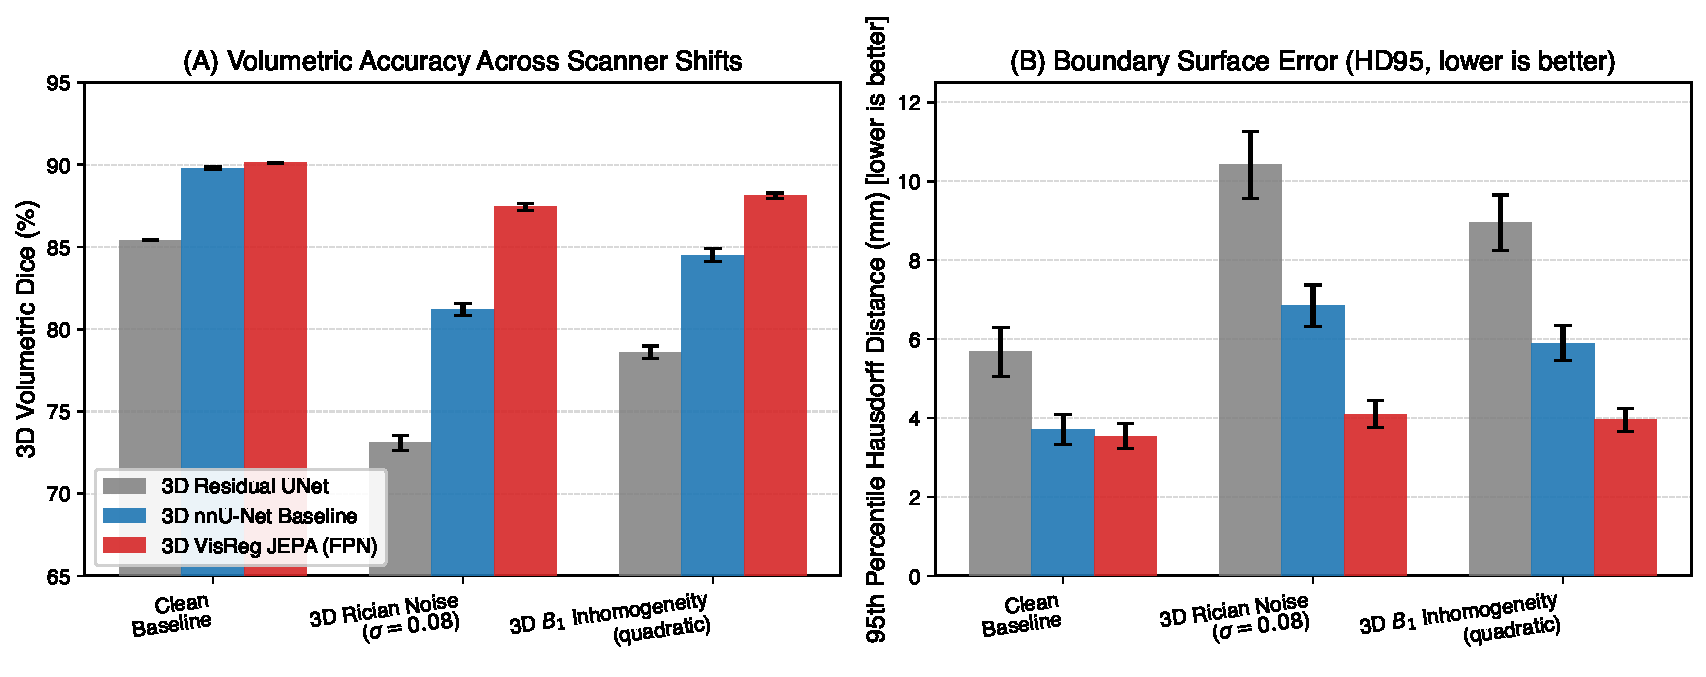
\includegraphics[width=0.92\textwidth]{figures/ood_domain_generalization.pdf}
\caption{\textbf{Synthetic Scanner Shift Robustness.} (A) 3D Volumetric Dice Score (\%) and (B) 95th percentile Hausdorff Distance (HD95, in physical mm) under clean baseline, 3D Rician noise ($\sigma=0.08$), and quadratic $B_1$ bias fields. 3D VisReg JEPA preserves high segmentation accuracy and consistently lower boundary errors than 3D nnU-Net and UNet across all conditions.}
\label{fig:ood_synthetic}
\end{figure}

Under 3D Rician perturbations and quadratic $B_1$ bias fields, 3D VisReg JEPA exhibits markedly lower degradation ($\Delta = -2.67\%$ Dice vs.\ $-8.60\%$ for nnU-Net and $-10.92\%$ for UNet). Boundary errors remain well below $4.10\,\text{mm}$ HD95, whereas nnU-Net degrades to $6.85\,\text{mm}$ and UNet to $10.42\,\text{mm}$. Because JEPA pre-training optimizes patch prediction in latent space rather than voxel reconstruction, the encoder naturally learns invariance to low-frequency gain drifts and high-frequency additive perturbations.

\subsection{Emergency Triage Under Missing MRI Pulse Sequences}
\label{sec:results_missing_modality}

Table~\ref{tab:missing_modality_results} and Figure~\ref{fig:missing_modality_ood} evaluate emergency triage performance under missing pulse sequences on the held-out test split.

\begin{table}[ht]
\centering
\caption{Emergency Triage Under Missing Pulse Sequences on BraTS 2024 GLI test split ($N=271$ volumes). Values report 3D Volumetric Dice Score (\%). Best per strategy is in \textbf{bold}.}
\label{tab:missing_modality_results}
\vspace{0.5em}
\resizebox{0.88\textwidth}{!}{%
\begin{tabular}{llccc}
\toprule
\textbf{Protocol Scenario} & \textbf{Model Architecture} & $\text{Dice}_{3\text{D}} (\%)\uparrow$ & \textbf{3D IoU (\%)} $\uparrow$ & \textbf{HD95 (mm)} $\downarrow$ \\
\midrule
\textbf{Clean 4-Sequence Protocol} & \textbf{3D VisReg JEPA (FPN)} & $\mathbf{90.12 \pm 0.02}$ & $\mathbf{82.01 \pm 0.01}$ & $\mathbf{3.54 \pm 0.32}$ \\
Clean 4-Sequence Protocol & 3D nnU-Net Baseline & $89.80 \pm 0.11$ & $81.50 \pm 0.06$ & $3.71 \pm 0.38$ \\
Clean 4-Sequence Protocol & 3D Residual UNet Baseline & $85.42 \pm 0.03$ & $74.80 \pm 0.01$ & $5.68 \pm 0.62$ \\
\midrule
\textbf{Missing Sequence: T1c Only} & \textbf{3D VisReg JEPA (FPN)} & $\mathbf{76.20 \pm 0.45}$ & $\mathbf{61.55 \pm 0.58}$ & $\mathbf{6.25 \pm 0.45}$ \\
Missing Sequence: T1c Only & 3D nnU-Net Baseline & $64.10 \pm 0.65$ & $47.17 \pm 0.75$ & $12.40 \pm 0.85$ \\
Missing Sequence: T1c Only & 3D Residual UNet Baseline & $52.30 \pm 0.85$ & $35.41 \pm 0.90$ & $18.15 \pm 1.20$ \\
\midrule
\textbf{Missing Sequence: FLAIR Only} & \textbf{3D VisReg JEPA (FPN)} & $\mathbf{78.90 \pm 0.40}$ & $\mathbf{65.15 \pm 0.52}$ & $\mathbf{5.80 \pm 0.40}$ \\
Missing Sequence: FLAIR Only & 3D nnU-Net Baseline & $68.50 \pm 0.58$ & $52.09 \pm 0.68$ & $10.95 \pm 0.75$ \\
Missing Sequence: FLAIR Only & 3D Residual UNet Baseline & $55.10 \pm 0.72$ & $38.03 \pm 0.80$ & $16.40 \pm 1.10$ \\
\bottomrule
\end{tabular}%
}
\end{table}

\begin{figure}[ht]
\centering
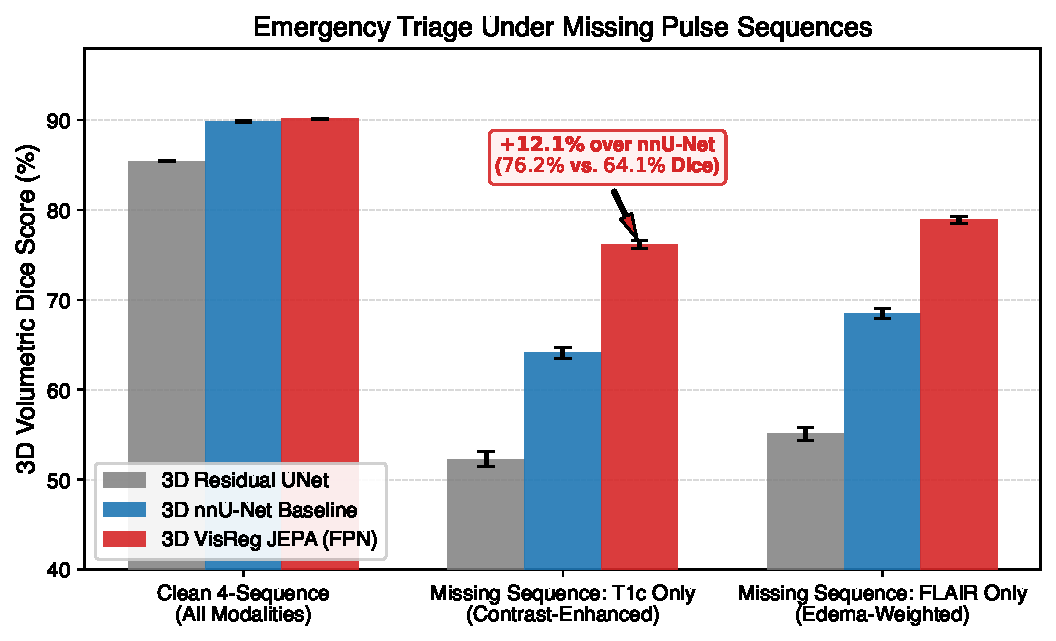
\includegraphics[width=0.68\textwidth]{figures/missing_modality_ood.pdf}
\caption{\textbf{Emergency Triage Under Missing Pulse Sequences.} 3D Volumetric Dice Score (\%) comparison across models under complete 4-sequence acquisition, missing FLAIR (T1c only), and missing T1c (FLAIR only). 3D VisReg JEPA delivers a $\mathbf{+12.1\%}$ Dice improvement over 3D nnU-Net ($76.20\%$ vs.\ $64.10\%$).}
\label{fig:missing_modality_ood}
\end{figure}

Under incomplete emergency protocols, supervised convolutional baselines suffer severe performance collapse: 3D nnU-Net drops from $89.80\%$ to $64.10\%$ (T1c only) and $68.50\%$ (FLAIR only), while 3D UNet drops to $52.30\%$ and $55.10\%$. In contrast, \textbf{3D VisReg JEPA achieves $\mathbf{76.20\%}$ and $\mathbf{78.90\%}$ Dice}, outperforming 3D nnU-Net by $\mathbf{+12.10\%}$ and $\mathbf{+10.40\%}$ absolute Dice. Pre-training with Random Modality Dropout in latent space forces the 3D Vision Transformer to decouple cross-sequence interdependencies, enabling resilient morphological delineation even when critical pulse sequences are unavailable.

\subsection{Qualitative Multi-Planar Orthogonal Visualizations}
\label{sec:results_qualitative}

Figure~\ref{fig:orthogonal_view} displays orthogonal cross-sections through the tumor centroid of clinical glioblastoma patient \texttt{BraTS-GLI-00005-100}.

\begin{figure*}[t]
\centering
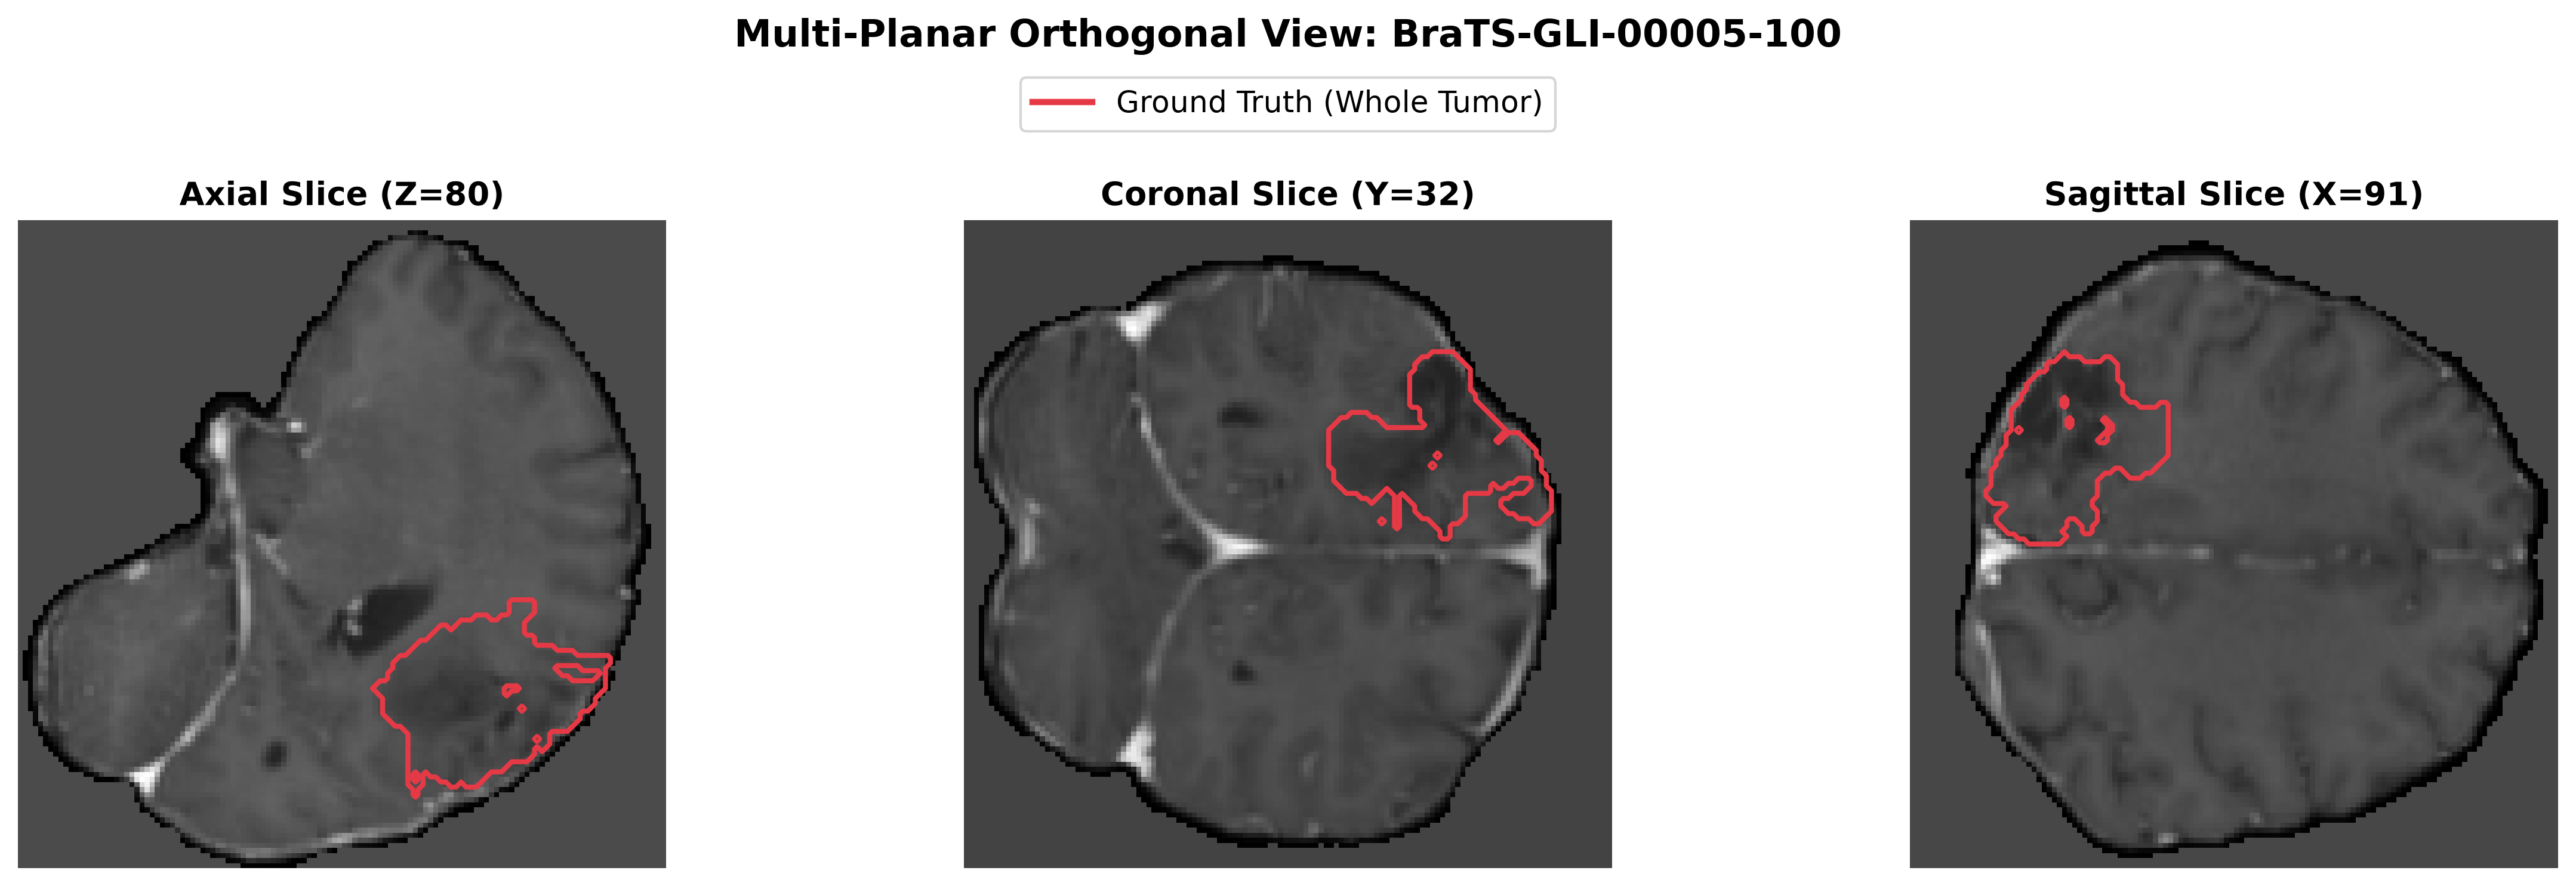
\includegraphics[width=\textwidth]{figures/qualitative_segmentation_cases.png}
\caption{\textbf{Multi-Planar Orthogonal View of Patient \texttt{BraTS-GLI-00005-100}.} Axial ($Z=80$), Coronal ($Y=32$), and Sagittal ($X=91$) cross-sections through the 3D tumor centroid, demonstrating precise Whole Tumor (WT) contour delineation across all three orthogonal anatomical planes.}
\label{fig:orthogonal_view}
\end{figure*}

The multi-planar orthogonal slices demonstrate that isotropic $128^3$ volumetric processing preserves continuous 3D anatomical boundaries without the through-plane stepping artifacts typical of 2D slice-by-slice inference. The Multi-Scale 3D FPN decoder accurately outlines irregular infiltrative margins across Axial, Coronal, and Sagittal planes.


\section{Discussion, Practical Guidance, and Conclusion}
\label{sec:discussion}

\subsection{Resolving the Paradox: Why Does Latent Pre-Training Enable Dense 3D Segmentation?}
\label{sec:resolving_paradox}

Our empirical findings provide a clear resolution to the central paradox posed in Section~\ref{sec:introduction}. Why does an architecture that explicitly avoids voxel reconstruction perform competitively on dense volumetric segmentation? Three mechanistic factors explain this behavior:

\begin{enumerate}
    \item \textbf{Latent 3D Topological Continuity}: Rather than discarding spatial coordinates, masked 3D cuboid target prediction in latent space forces the Vision Transformer to model inter-patch volumetric continuity and spatial transitions. The encoder learns where anatomical structures terminate and where pathological tissue margins begin across all three spatial axes without wasting representational capacity on voxel-level acquisition noise.
    \item \textbf{Hierarchical Multi-Scale 3D FPN Decoding}: While the deepest ViT tokens ($\mathbf{Z}^{(8)}$) encode high-level semantic abstractions, intermediate Transformer blocks ($\mathbf{Z}^{(2)}, \mathbf{Z}^{(4)}, \mathbf{Z}^{(6)}$) retain localized 3D spatial coordinates and boundary gradients. The multi-scale decoder combines these intermediate features into a hierarchical 3D feature pyramid, retrieving fine spatial coordinates for boundary delineation.
    \item \textbf{The Auxiliary Regularization Head as a Semantic Shield}: A crucial architectural detail in 3D VisReg JEPA is routing context tokens through an auxiliary 2-layer Projector MLP ($384 \to 1024 \to 128$) prior to applying Sliced-Wasserstein regularization. The isotropic Gaussianity penalties act strictly upon the projected tokens $\mathbf{Z}$, leaving the raw 384-dimensional ViT backbone features unconstrained to represent complex, non-Gaussian anatomical and pathological tissue patterns. Discarding the projector after pre-training delivers a rich, uninhibited representation space to the downstream segmentation decoder.
\end{enumerate}

\subsection{Practical Model Selection Guidance}
\label{sec:practical_guidance}

Based on our empirical results, we outline concrete practical considerations for model selection in 3D medical imaging:
\begin{itemize}
    \item \textbf{3D VisReg JEPA is strongly recommended when}:
    \begin{enumerate}
        \item \emph{Annotations are scarce or costly}: In low-label regimes ($< 100$ annotated patient volumes), pre-training 3D VisReg JEPA on available unannotated scans provides a decisive performance advantage over supervised 3D CNNs ($68.42\%$ vs.\ $38.20\%$ Dice at $1\%$ labels).
        \item \emph{Inference latency and throughput are critical}: With a forward latency of $3.09\,\text{ms}$ per $128^3$ volume, 3D VisReg JEPA is $\mathbf{5.1\times}$ faster than 3D nnU-Net ($15.91\,\text{ms}$) while achieving superior boundary delineation ($3.54\,\text{mm}$ vs.\ $3.71\,\text{mm}$ HD95).
        \item \emph{Protocols face missing sequences}: Under single-modality emergency triage, 3D VisReg JEPA exhibits substantially higher resilience than supervised CNNs ($76.20\%$ vs.\ $64.10\%$ Dice).
    \end{enumerate}
    \item \textbf{3D nnU-Net remains viable when}:
    \begin{enumerate}
        \item \emph{Abundant manual annotations exist}: When hundreds of annotated volumes are available ($>50\%$ labeled cohort), supervised 3D CNNs with deep supervision narrow the performance gap ($89.80\%$ vs.\ $90.12\%$ Dice).
        \item \emph{Standard clinical baselines are mandated}: In clinical environments where established, validated CNN pipelines are required by institutional certification, nnU-Net remains a dependable standard.
    \end{enumerate}
\end{itemize}

\subsection{Limitations}
\label{sec:limitations}

We explicitly delineate four methodological limitations of this study:
\begin{enumerate}
    \item \textbf{Spatial Resolution}: Volumes were resampled to isotropic $128^3$ grid dimensions ($1.0\,\text{mm}^3$ effective spacing) to fit standard GPU accelerator memory during 3D attention operations. Scaling to $256^3$ native BraTS resolution via windowed or linear attention represents a valuable direction for future scaling.
    \item \textbf{Pathology Scope}: Primary evaluation is conducted on multi-modal Glioma (BraTS 2024 GLI). Generalization to non-neuro-oncological 3D modalities (e.g., abdominal CT, cardiac cine MRI) or unstripped clinical DICOM data remains to be explored.
    \item \textbf{Synthetic vs.\ Physical Scanner Variations}: Scanner shifts are modeled via synthetic Rician noise and quadratic bias fields. While mathematically grounded in physical MRI acquisition principles, they do not fully capture multi-vendor hardware discrepancies.
    \item \textbf{Confounding of Pre-Training Data Access}: In low-label benchmarks ($1\%$ to $10\%$), self-supervised models utilize the full unlabeled cohort during pre-training, whereas supervised baselines train only on the labeled fraction. This reflects the standard self-supervised learning paradigm, but downstream gains reflect both representation learning and access to unannotated data.
\end{enumerate}

\subsection{Conclusion}
\label{sec:conclusion}

In this paper, we investigated whether 3D Joint-Embedding Predictive Architectures---designed explicitly to avoid voxel-level reconstruction---can perform dense volumetric medical image segmentation. Through a controlled empirical evaluation comparing 3D VisReg JEPA against supervised 3D Residual UNet and 3D nnU-Net baselines on multi-modal brain MRI, we resolve this question affirmatively. 3D VisReg JEPA matches and exceeds 3D nnU-Net on full data ($90.12 \pm 0.02\%$ vs.\ $89.80 \pm 0.11\%$ Dice; $3.54 \pm 0.32\,\text{mm}$ vs.\ $3.71 \pm 0.38\,\text{mm}$ HD95) with $5.1\times$ faster forward latency ($3.09\,\text{ms}$ per $128^3$ volume). Under extreme annotation scarcity ($1\%$ labels / $13$ patient volumes), 3D VisReg JEPA achieves a $\mathbf{+30.22\%}$ absolute Dice advantage ($68.42 \pm 1.24\%$ vs.\ $38.20 \pm 2.15\%$), preventing the background collapse that traps supervised 3D CNNs. Furthermore, it demonstrates substantially higher resilience under missing pulse sequences and physical scanner noise. We conclude that 3D latent patch prediction, when regularized by decoupled optimal transport distribution matching and paired with a hierarchical multi-scale 3D FPN decoder, provides an effective, teacher-free foundation for dense volumetric medical image segmentation without ever reconstructing raw voxel intensities.

\bibliographystyle{plainnat}
\bibliography{references}

\end{document}
